%!TEX root = ../report.tex


\chapter{Design}\label{ch:design}

\section{Design artefacts}\label{sec:design-artefacts}

This part of the document will present the artefacts which have been developed during the design phase.

\begin{figure}[h]
    \centering
    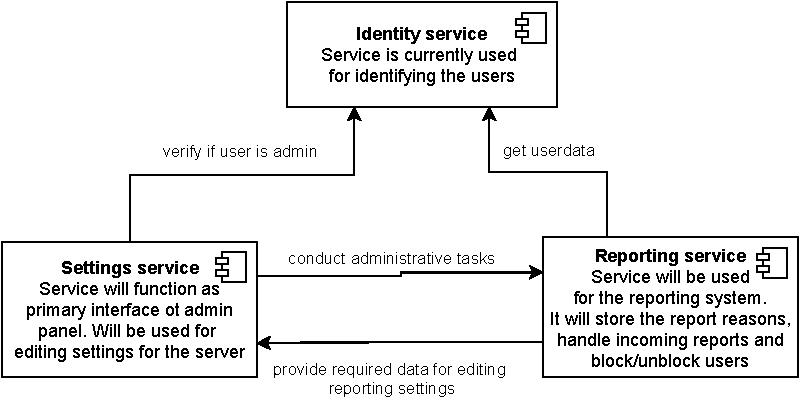
\includegraphics[width=1.0\textwidth]{./graphics/component_interaction}
    \caption{Service interaction concept designed for admin panel}
    \label{fig:componentInteraction}
\end{figure}

Figure~\ref{fig:componentInteraction} shows a concept for the components that will have to be added for the admin panel.
The Settings service will function as the rest interface to the Admin panel.
To this point it will interact with the identity service for verifying if the settings are actually being changed by an
administrator user.
It will also work with the reporting service, which is also another new service in charge of handling the reporting
system, to conduct administrative tasks like changing the reasons people can be reported for.

\begin{figure}[h]
    \centering
    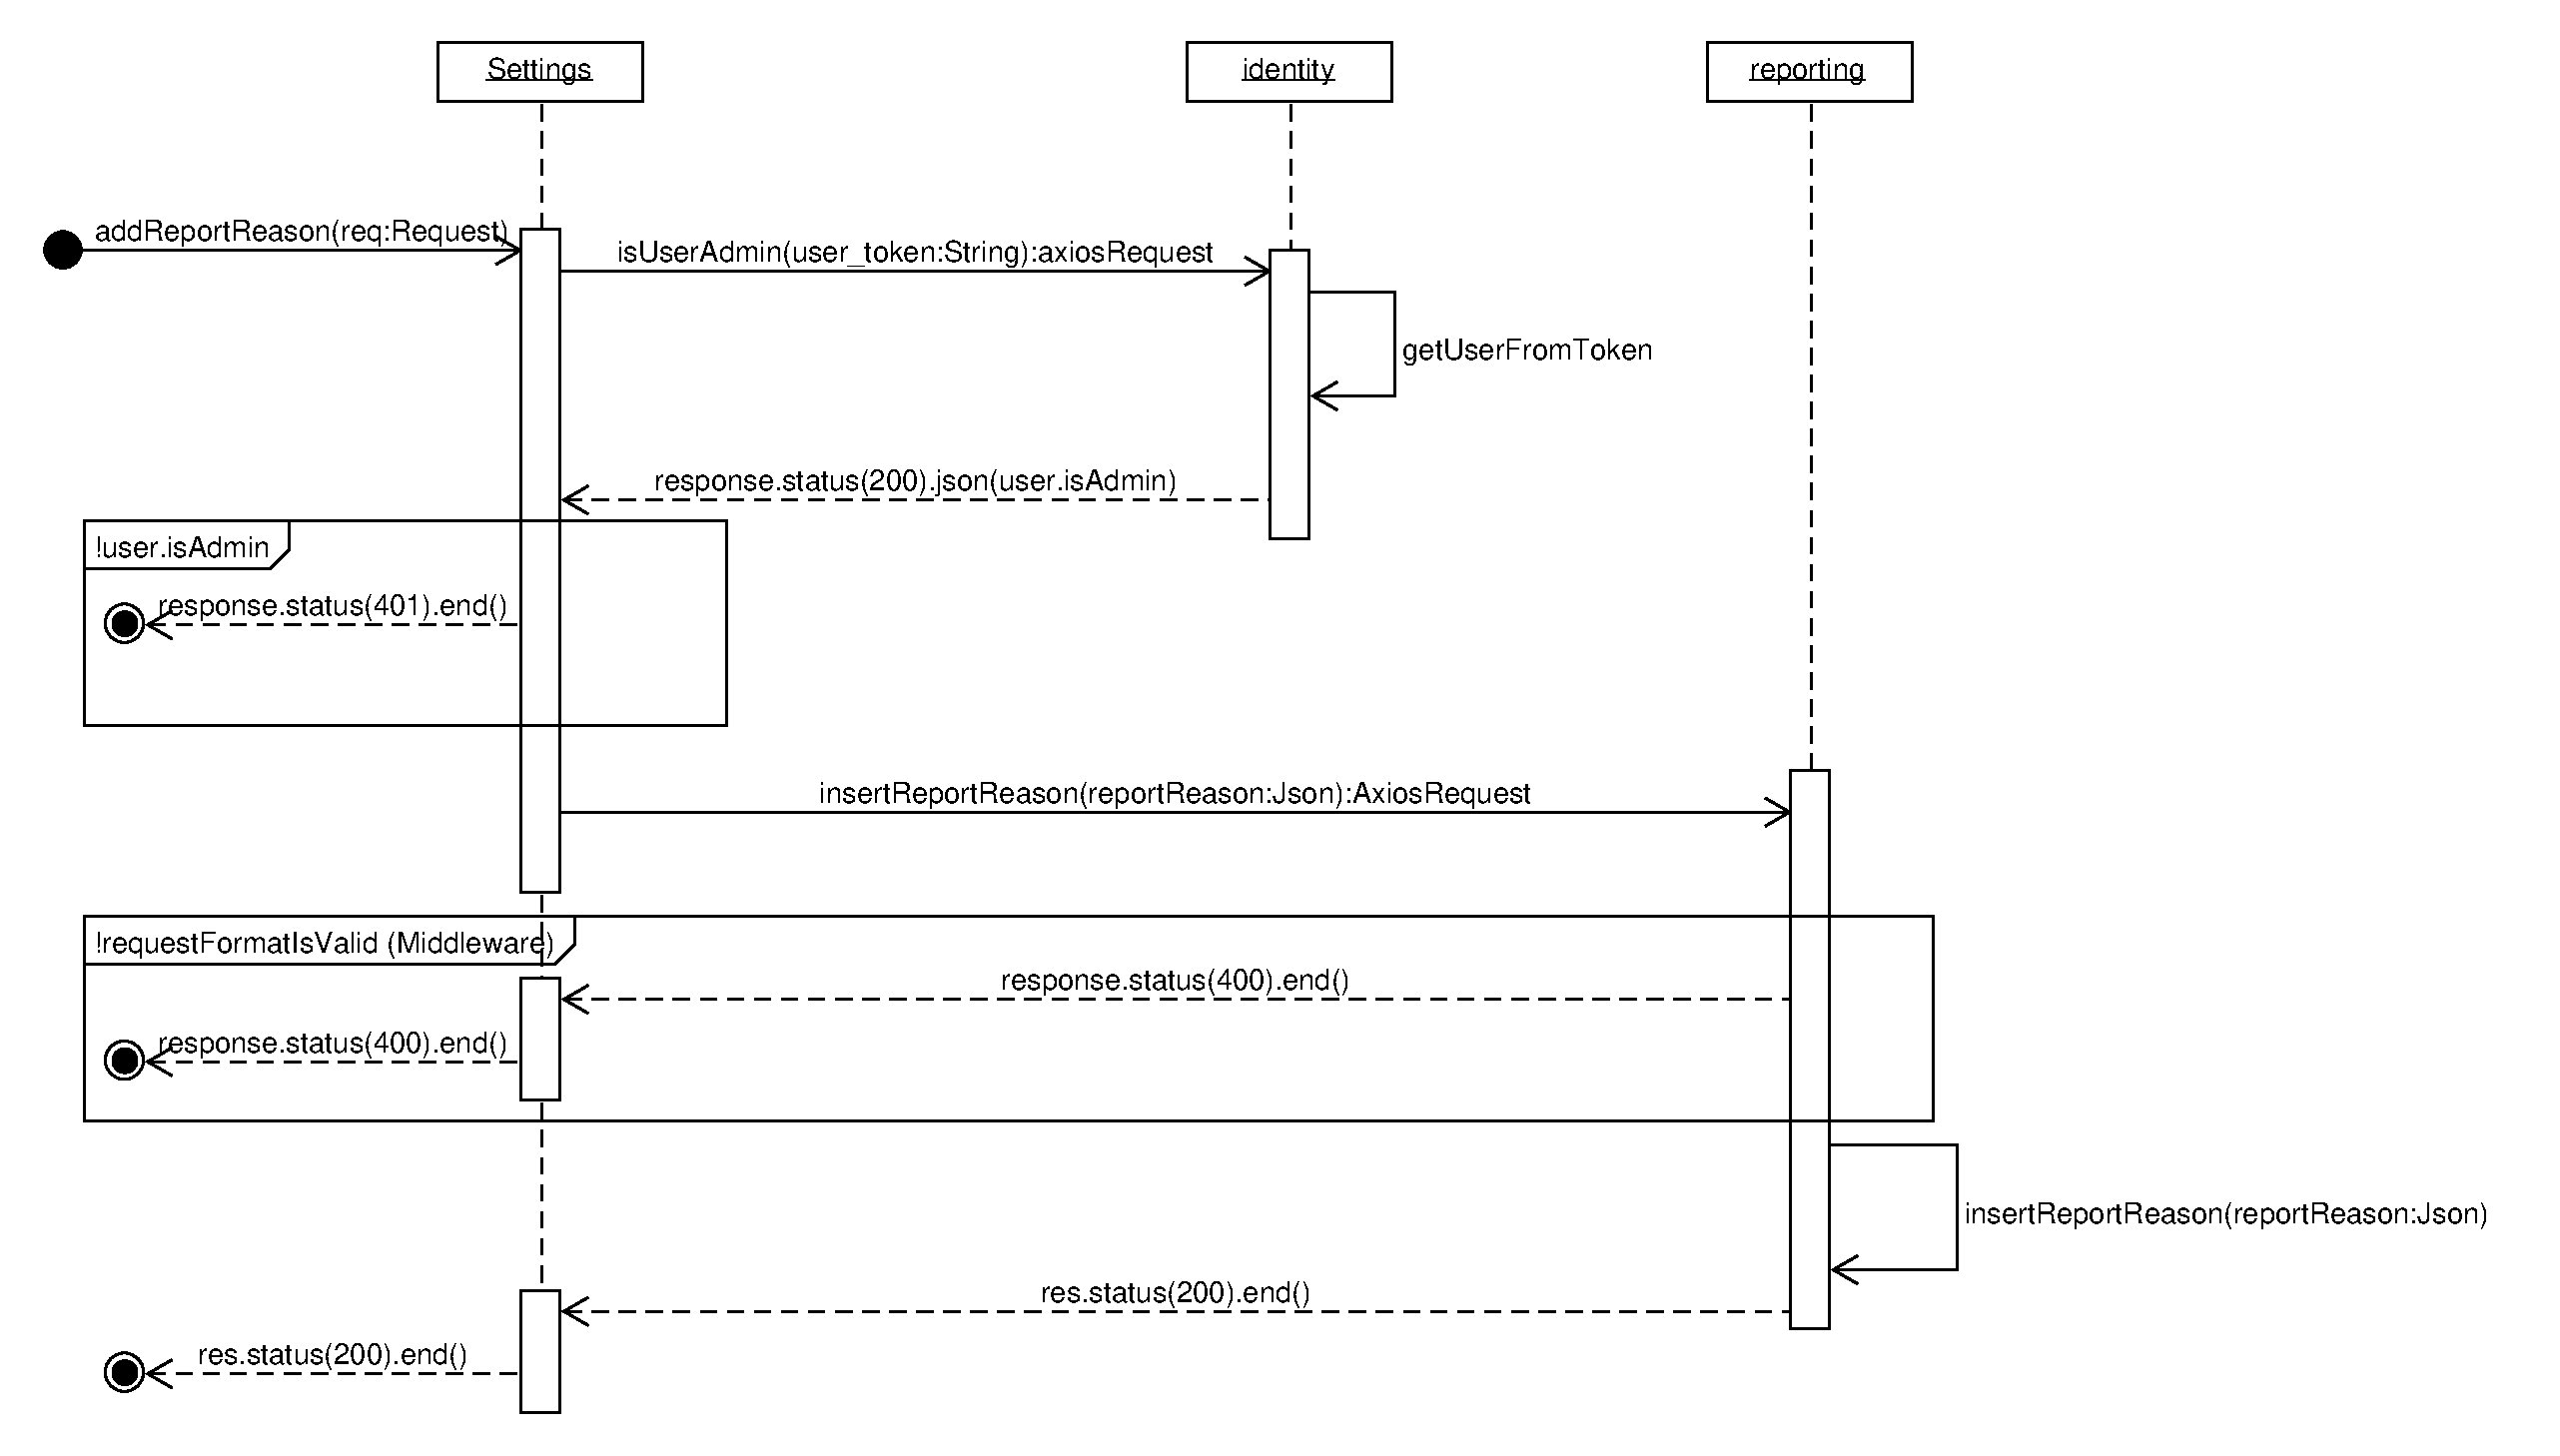
\includegraphics[width=1.0\textwidth]{./graphics/SequenceDiagram_AddReportReason}
    \caption{Service interaction concept designed for admin panel}
    \label{fig:sequenceDiagramAddReportReason}
\end{figure}

Figure~\ref{fig:sequenceDiagramAddReportReason} shows the sequence diagram for conducting the administrative task of
adding a report reason.
This diagram has been created in order to further visualize the responsibility and interaction between the existing
identity service, and the two new services (settings and reporting).
Further information on this can be derived from~\hyperref[subsubsec:settingsSer]{\textbf{settings service}}.

\begin{figure}[h]
    \centering
    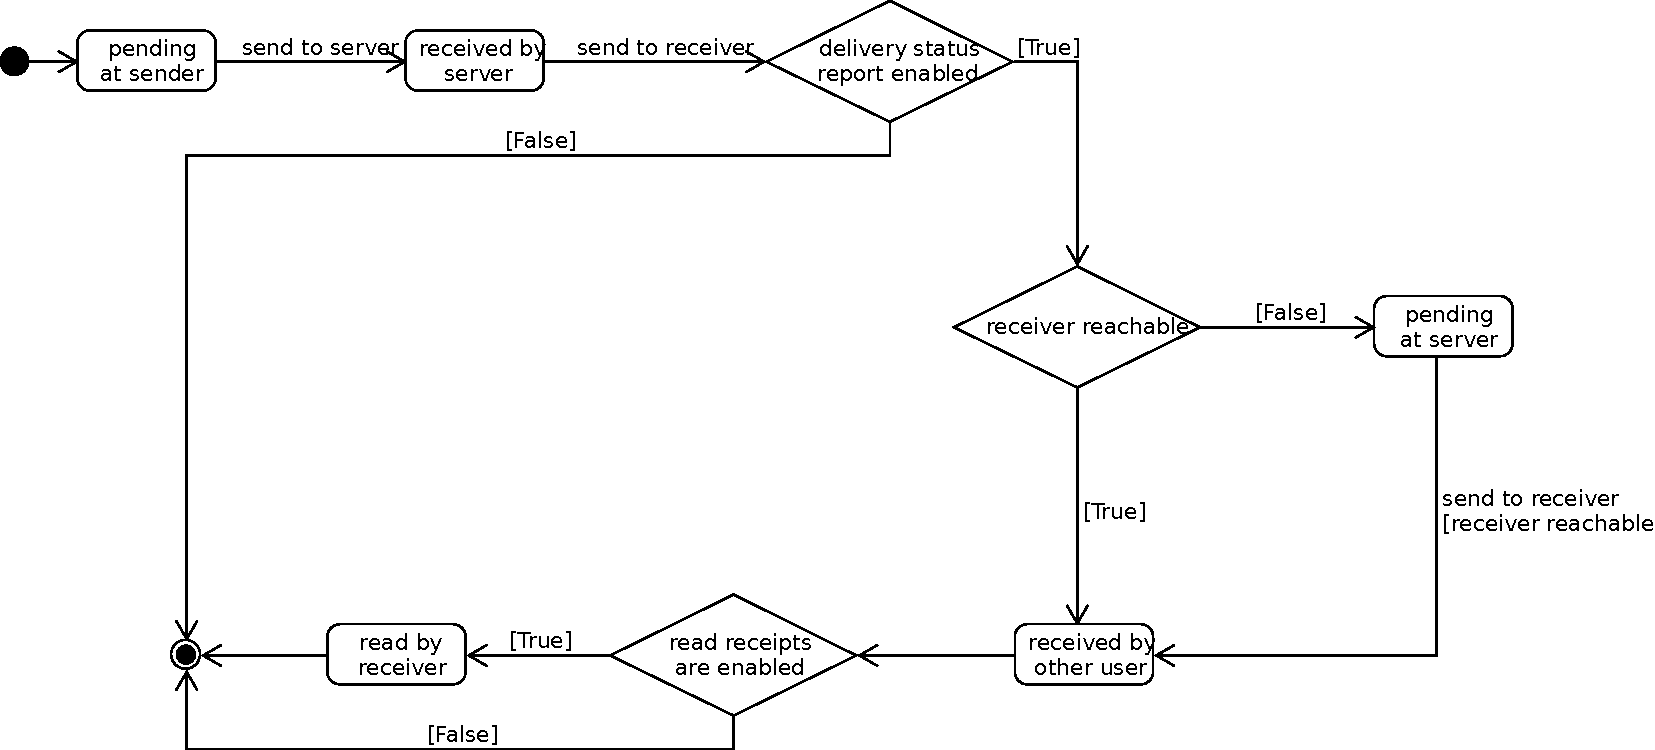
\includegraphics[width=1.0\textwidth]{./graphics/stateMachineMessage}
    \caption{State machine diagram for the message}
    \label{fig:stateMachineMessage}
\end{figure}

Figure~\ref{fig:stateMachineMessage} shows the different states of the message.
First the message will be in the pending at sender stage, once the message has been successfully sent to the server,
it will enter the \enquote{received by server}.
From there on it depends on the settings of the user, whether the delivers status report is enabled or not.
Should this option be disabled, the diagram ends here, otherwise, it will be checked if the receiver is reachable or
not.
If he is not reachable the state will be set to \enquote{pending at server} until the message was received by the intended
user, in which case the state will jump to \enquote{received by other user}.
Should the other user be immediately reachable, the state of the message will immediately jump to the received by other
user state.
Next it again depends on the settings, whether read receipts are enabled or not.
If they are not enabled the diagram ends here, otherwise the message state will be set to \enquote{read by receiver}
and the diagram ends here.

\begin{figure}[h]
    \centering
    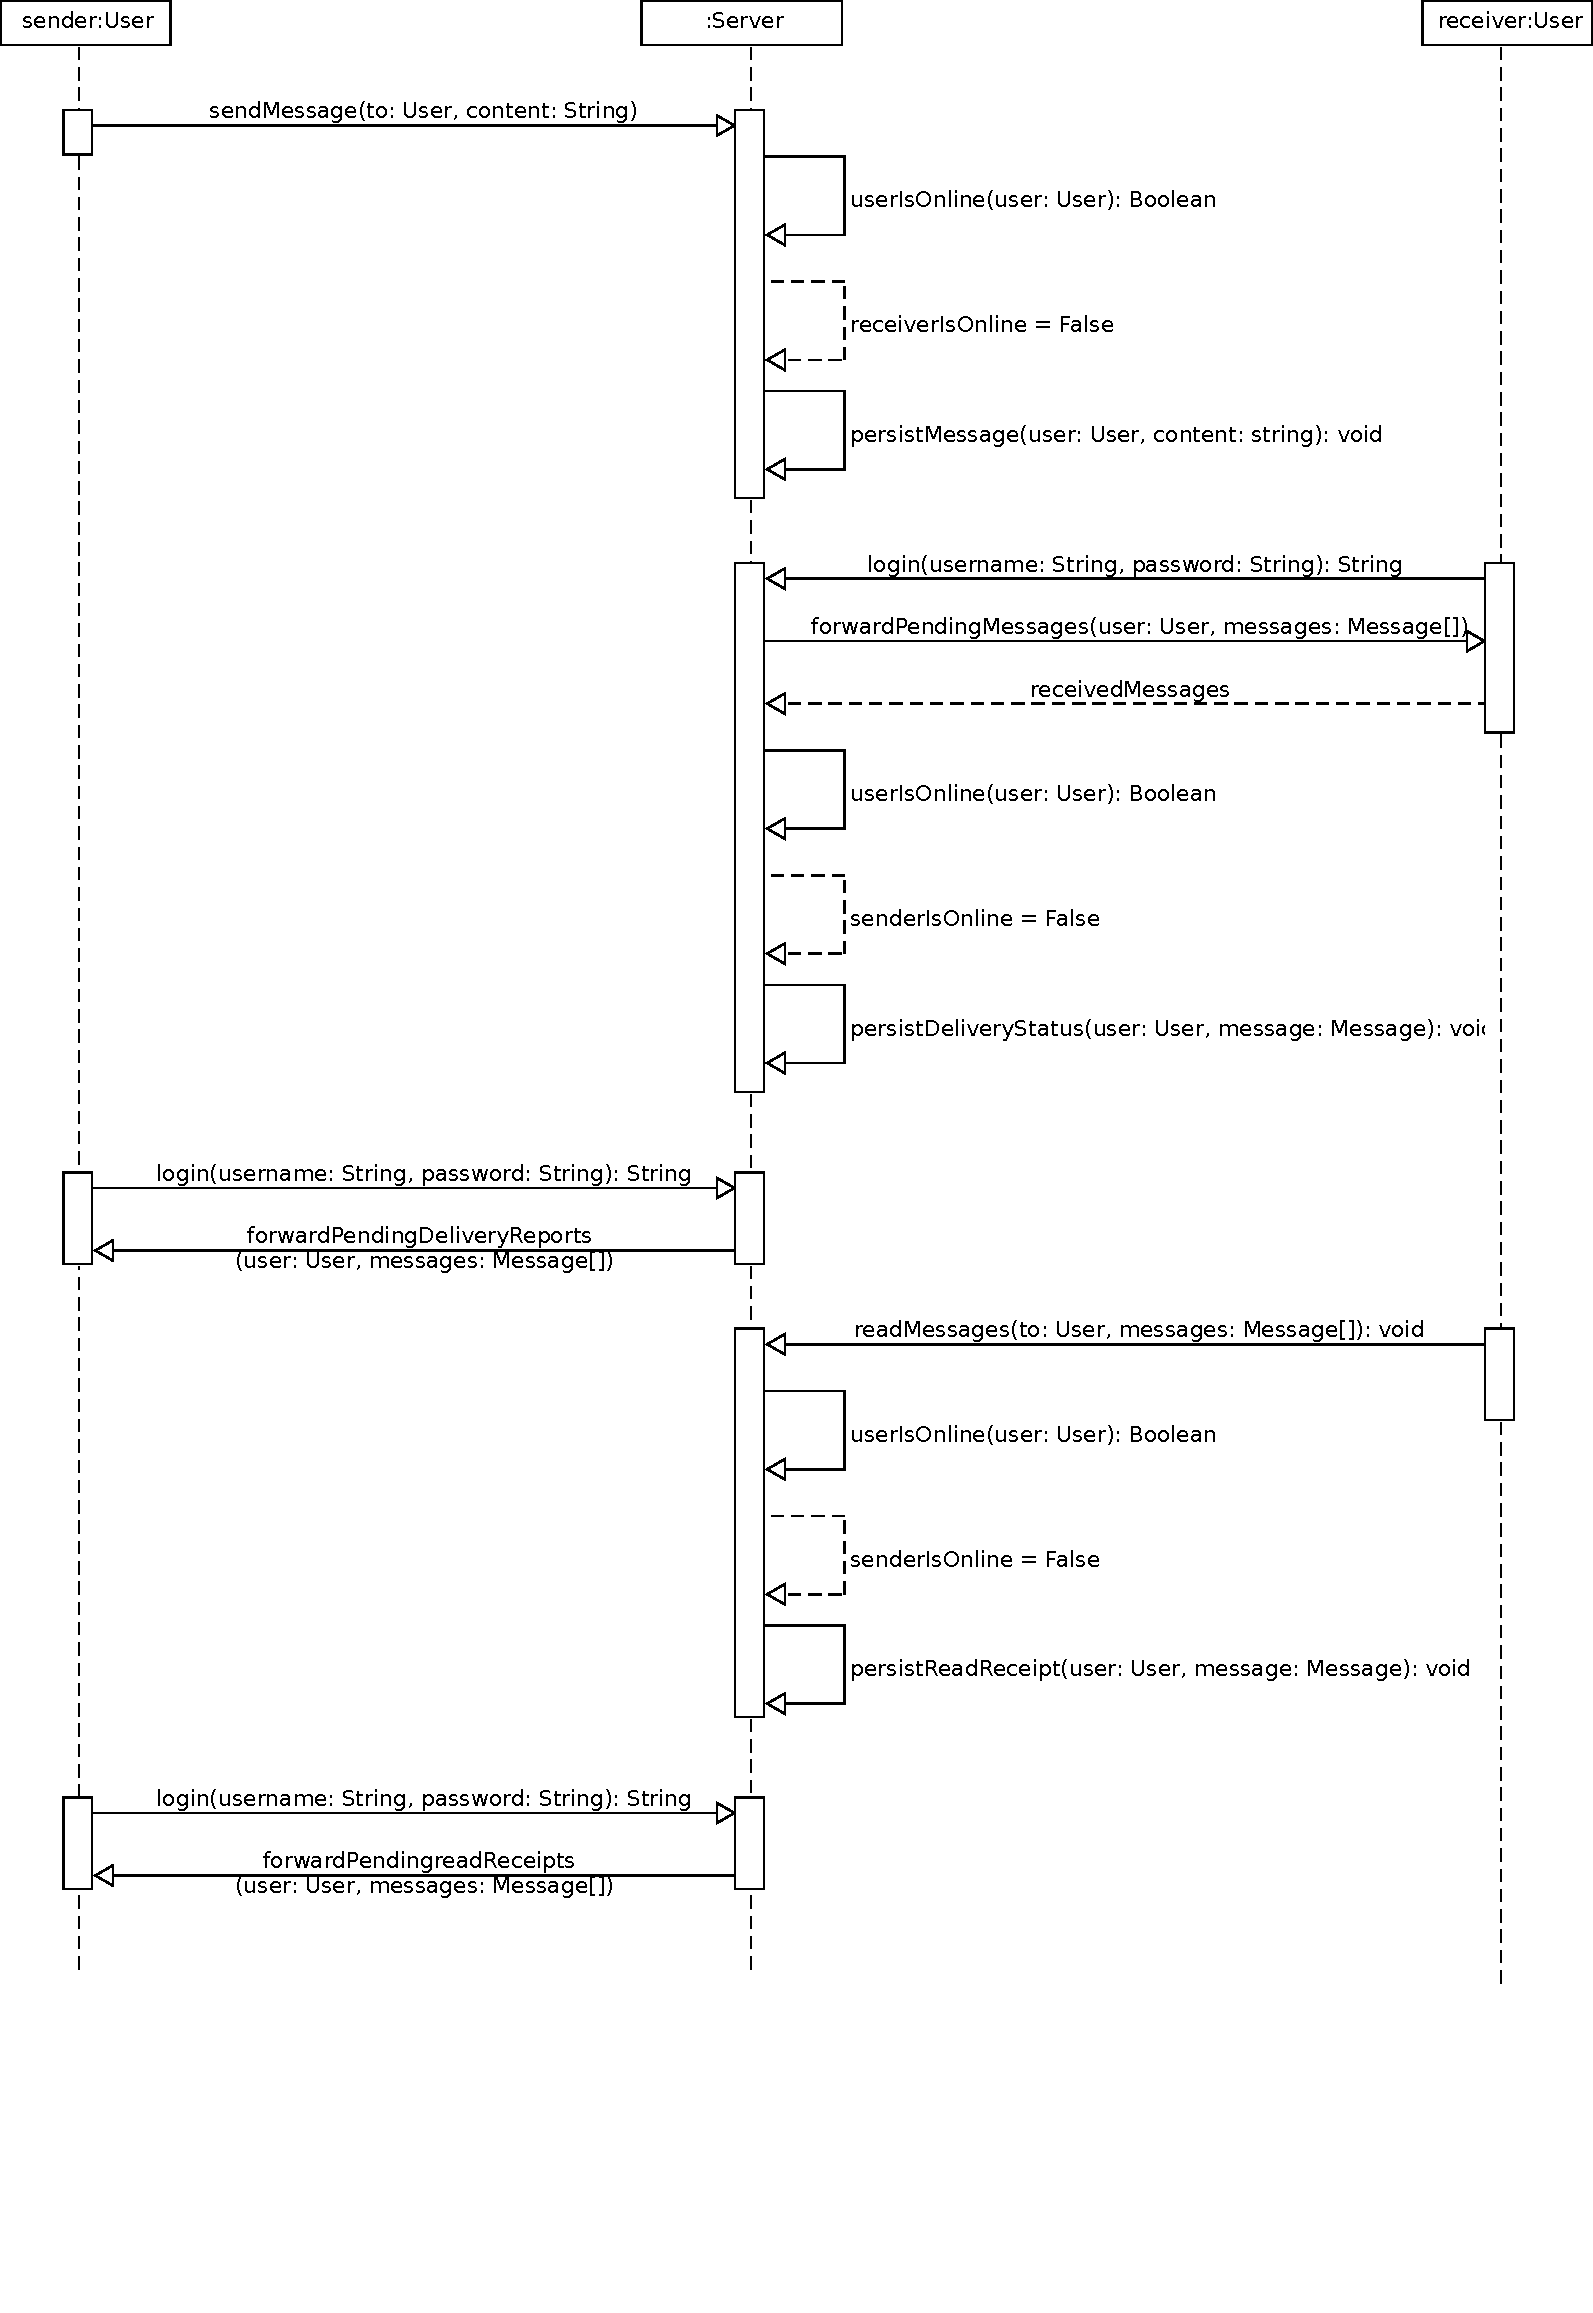
\includegraphics[width=1.0\textwidth]{./graphics/sequenceDiagramMessage}
    \caption{Sequence diagram for sending messages}
    \label{fig:sequenceDiagramMessage}
\end{figure}

Figure~\ref{fig:sequenceDiagramMessage} shows the sequence of sending a message.
This diagram will assume that all the worst cases (receiver is not online for receiving the message and sender is not
there for receiving status updates on the receipt and read receipt status of the message) in order to present how
forwarding of this information will be handled.
The sender sends the message with a certain receiver (to) and message (content).
The server then again checks if the receiver is online.
In this case he is not (receiverIsOnline = false).
The server will now temporarily store the message (persistMessage) until the receiver has logged in.
This will trigger the server to forward the pending messages to the receiver.
The receiver client will then let the server know that the message has been received.
The server will now check if the original user is online to forward the status update of the message.
In this case the original sender is offline (senderIsOnline = false).
The server will now again temporarily store the message status.
Once the sender has logged in, this will prompt the server to forward the delivery status to the sender.
The sender at a later point in time will read the message and forward this status to the server.
The server will check if the sender is online which he in this case again is not.
Once the sender is logged in the sender will then be forwarded the read receipt status by the server.

\section{Network Design}\label{sec:network-design}

\subsection{Application Layers}\label{subsec:application-layers}
% TODO @joernneumeyer & @mauritsvanderzee

\subsection{Network Architecture}\label{subsec:network-architecture}
% TODO @joernneumeyer & @mauritsvanderzee
% Umlet diagrams ..?

\subsection{Port distribution}\label{subsec:port-distribution}

% TODO @all add descrptions to table
\begin{table}[]
    \begin{tabular}{lll}
        \textbf{Port} & \textbf{Service}                               & \textbf{Description} \\
        8086          & Default Application Port                       & TODO @all            \\
        3000          & Identity Service                               & TODO @all            \\
        3001          & Chat service over HTTP                         & TODO @all            \\
        3002          & Chat service over SocialStuff/Trale connection & TODO @all
    \end{tabular}\label{tab:table}
\end{table}

\subsection{Database management system}\label{subsec:database-management-system}
% TODO @all Which dbms, why, schemas, which tables columns constraints etc.

\lipsum[2-4]
